\section{Architektur}

\section{Systemübersicht}

\section{Logische Architektur}
\begin{itemize}
	\item services: Web-Schnittstelle (RESTful)
	\item genericapi: Abstraktion für Compute, Storage und Network
	\item util: Tools zur Bearbeitung von Configfiles
	\item presistence: OR-Mapping
\end{itemize}

\begin{center}
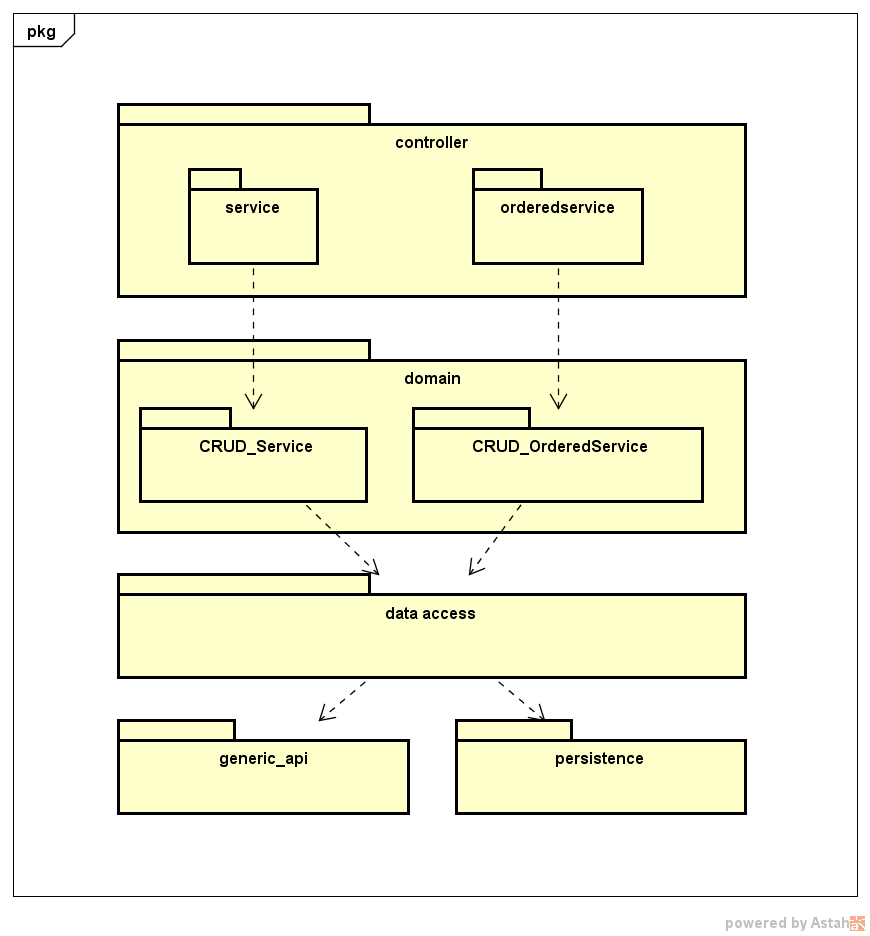
\includegraphics[width=\textwidth]{./05_Design/04_Architektur/LogischeSicht}
\end{center}

\newpage

\section{Klassenstruktur}

\subsection{services}

In der Schicht services wird die RestAPI implementiert.

\begin{center}
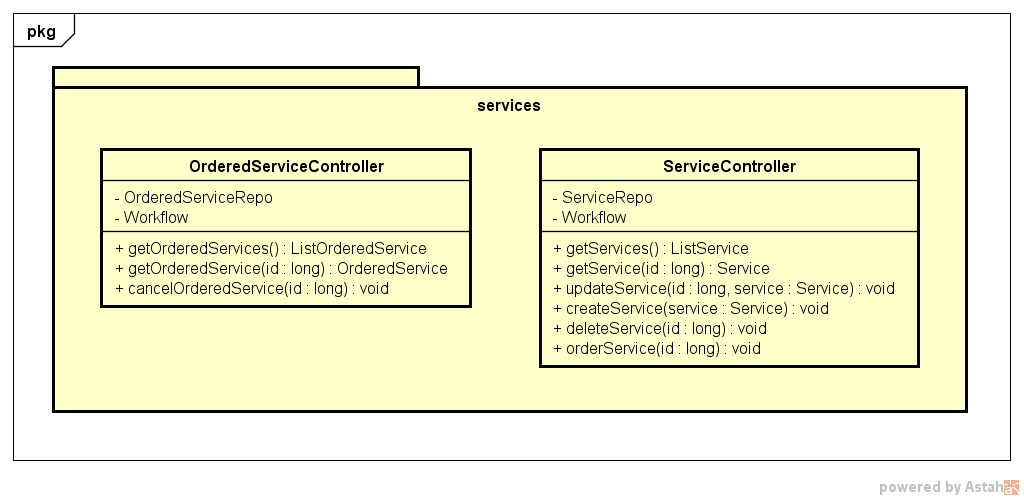
\includegraphics[width=\textwidth]{./05_Design/04_Architektur/services}
\end{center}

\subsection{domain}

Die Domain beinhaltet die Entitäten, die mittels OR-Mapper mit der Datenbank synchronisiert werden.
Der Workflow erstellt/löscht einen Service.

\begin{center}
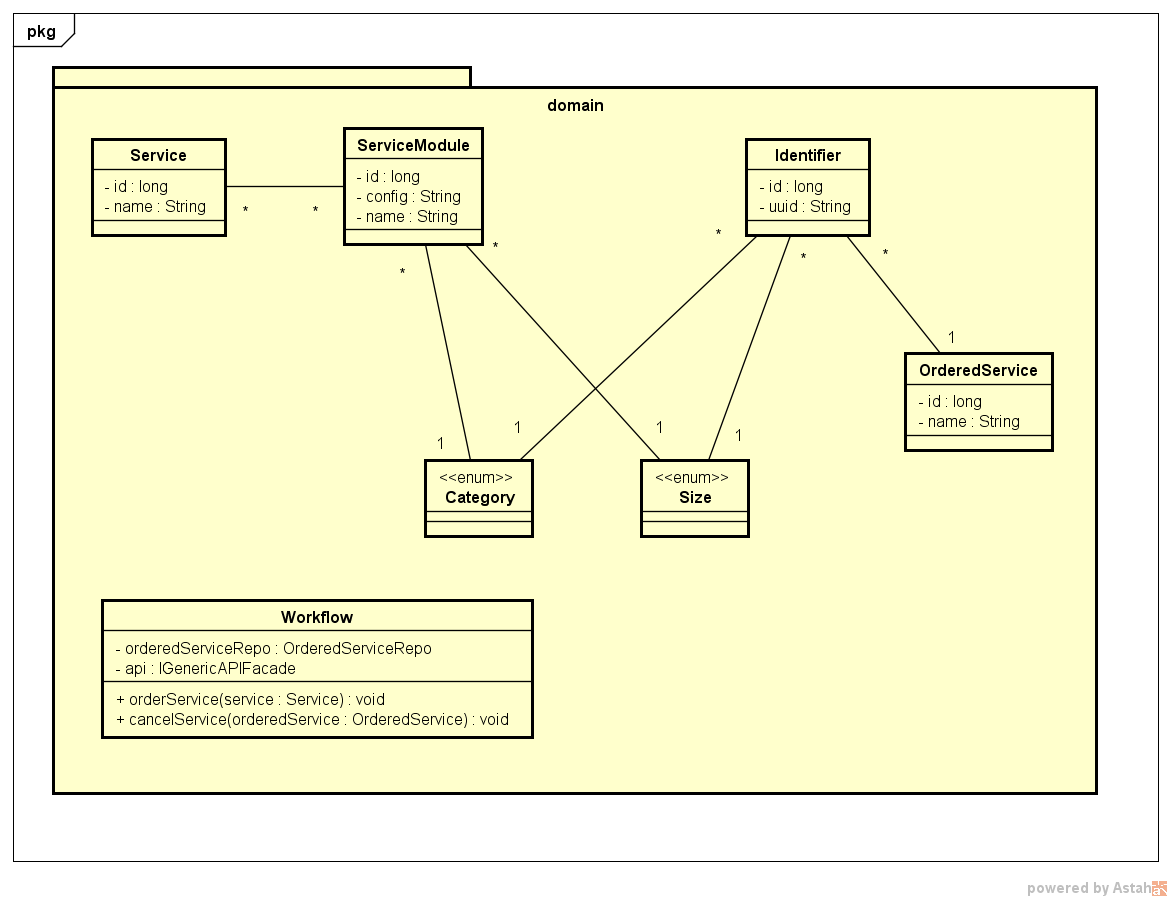
\includegraphics[width=\textwidth]{./05_Design/04_Architektur/domain}
\end{center}

\subsection{GenericAPI}
\subsubsection{ServiceModuleHandler}
Der ServiceModuleHandler entscheidet an welchen ResourceController ein ServiceModule/Identifier übergeben wird.
Der Entscheidungsalgorithmus kann auf verschiedenste Arten implementiert werden, deshalb gibt es ein Interface.

\subsubsection{ResourceController}
Der ResourceController ist eine Abstraktion eines Controllers, die nicht auf irgendwelche 
Bibliotheksabhängigkeiten (z.B. LibVirt, JClouds) eingeht und lediglich dem ServiceModuleHandler die nötigen Informationen anbietet.

\subsubsection{LibVirtController}
Der LibVirtController ist eine weitere Abstraktion eines Controllers, die aber speziell einer 
Bibliothek (in diesem Fall LibVirt) zugewiesen ist. Die Klasse kümmert sich um die 
Instanzierung und kann, wenn nötig, Helfermethoden anbieten.

\subsubsection{LibVirt<category>Controller}

Die konkrete Klasse des Controllers implementiert nur noch die abstrakten Methoden des ResourceControllers.

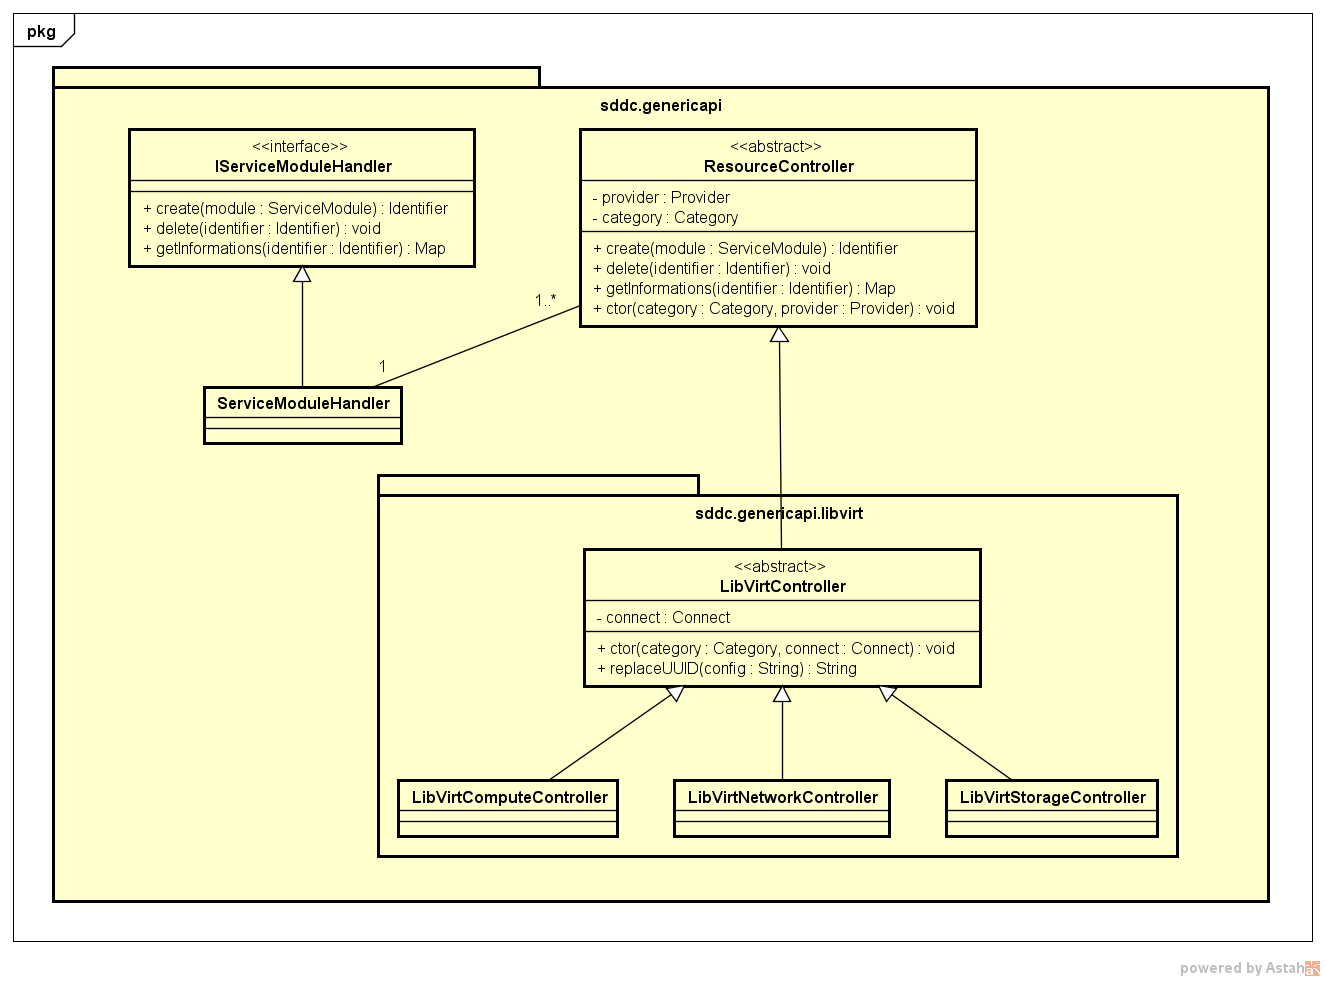
\includegraphics[width=\textwidth]{./05_Design/04_Architektur/genericapi}


\section{Dependency Injection}

Die GenericAPI ist relativ komplex ausgefallen und kann erweitert werden. Um unnötigen 
Code in den oberen Schichten zu vermeiden, wird die GenericAPI mit Hilfe von Dependency
 Injection aufgesetzt. Es ist möglich in einem XML die gesamte GenericAPI nach belieben zusammenzusetzen.

\section{Deployment}

Spring liefert einen Application Server mit, bei welchem es sich um einen Tomcat 
Server handelt. Der Datenbankserver wird über den JDBC Treiber angesprochen.

\includegraphics[width=\textwidth]{./05_Design/04_Architektur/deployment}

\section{Persistierung}
Für die Persistierung wird ein OR Mapper verwendet, wodurch die Java 
Objekte auf die Datenbank abgebildet werden.

\subsection{Service}
Der Service wird mit einer automatisch generierten ID und einem Namen 
abgespeichert, dabei ist der Name des Service Unique und kann nur einmal 
verwendet werden, was das auffinden eines Service vereinfacht.

\subsection{Servicemodule}
Das Servicemodul wird mit einer automatisch generierten ID abgespeichert und besitzt einen 
Namen (zur Identifizierung Unique).
Category, Size und Provider sind Enums und geben feste Werte vor z.B.: Size: 
S,M,L.
Das Configfile ist ein Text, wodurch es keine Rolle Spielt ob nun ein \ac{XML}, \ac{JSON} 
oder \ac{YAML} abgespeichert wird.

\subsection{Orderedservice}
Der Orderedservice besitzt eine automatisch generierte ID + einen nicht Uniquen 
Namen, um einen Service auch mehrfach abonnieren zu können.

\subsection{Identifier}
Der Identifier besitzt eine generierte ID + den Namen des dazugehörigen 
Servicemodul.
Kategorie, Size und Provider werden ebenfalls vom Servicemodul übernommen.
Die uuid ist je nach Provider verschieden und wird durch diesen vorgegeben.

\subsection{Identifier Infos}
Die Identifier Infos beinhalten die vorhanden Infos zu einem abonnierten 
Servicemodul, welche auf dem Dashboard ausgegeben werden.

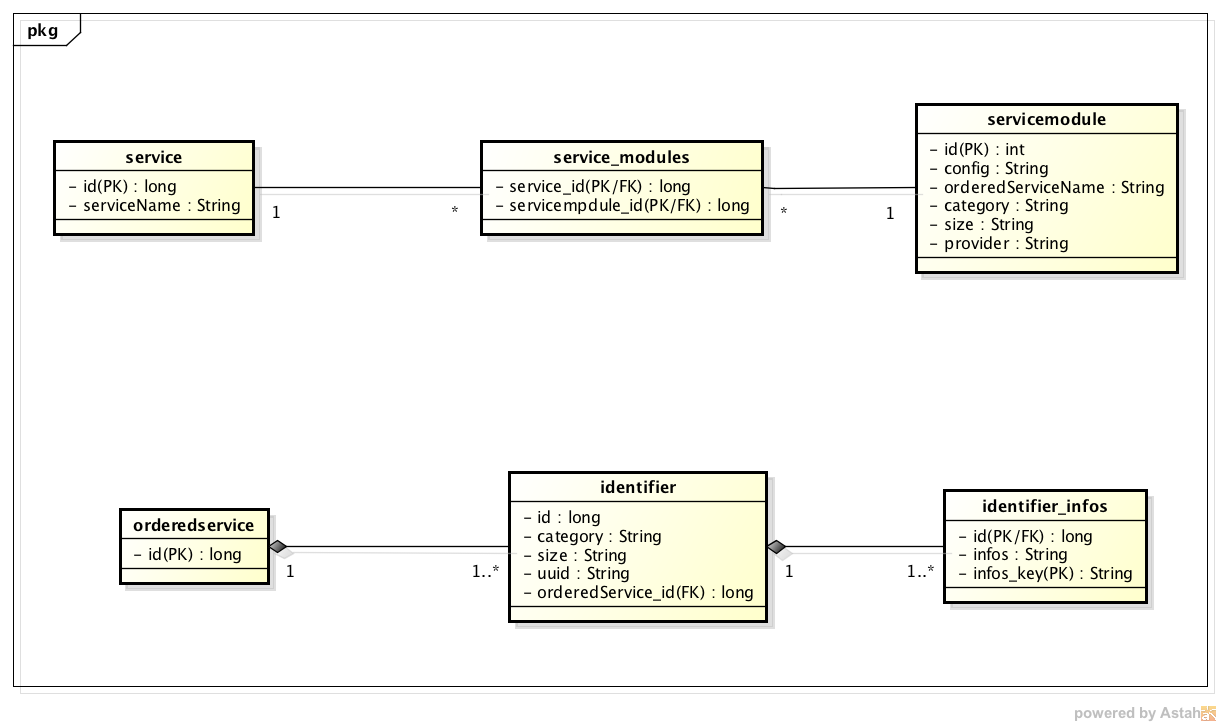
\includegraphics[width=\textwidth]{./05_Design/04_Architektur/Datenmodell}

\section{Sequenzdiagramme}
\subsection{service bestellen}

\begin{center}
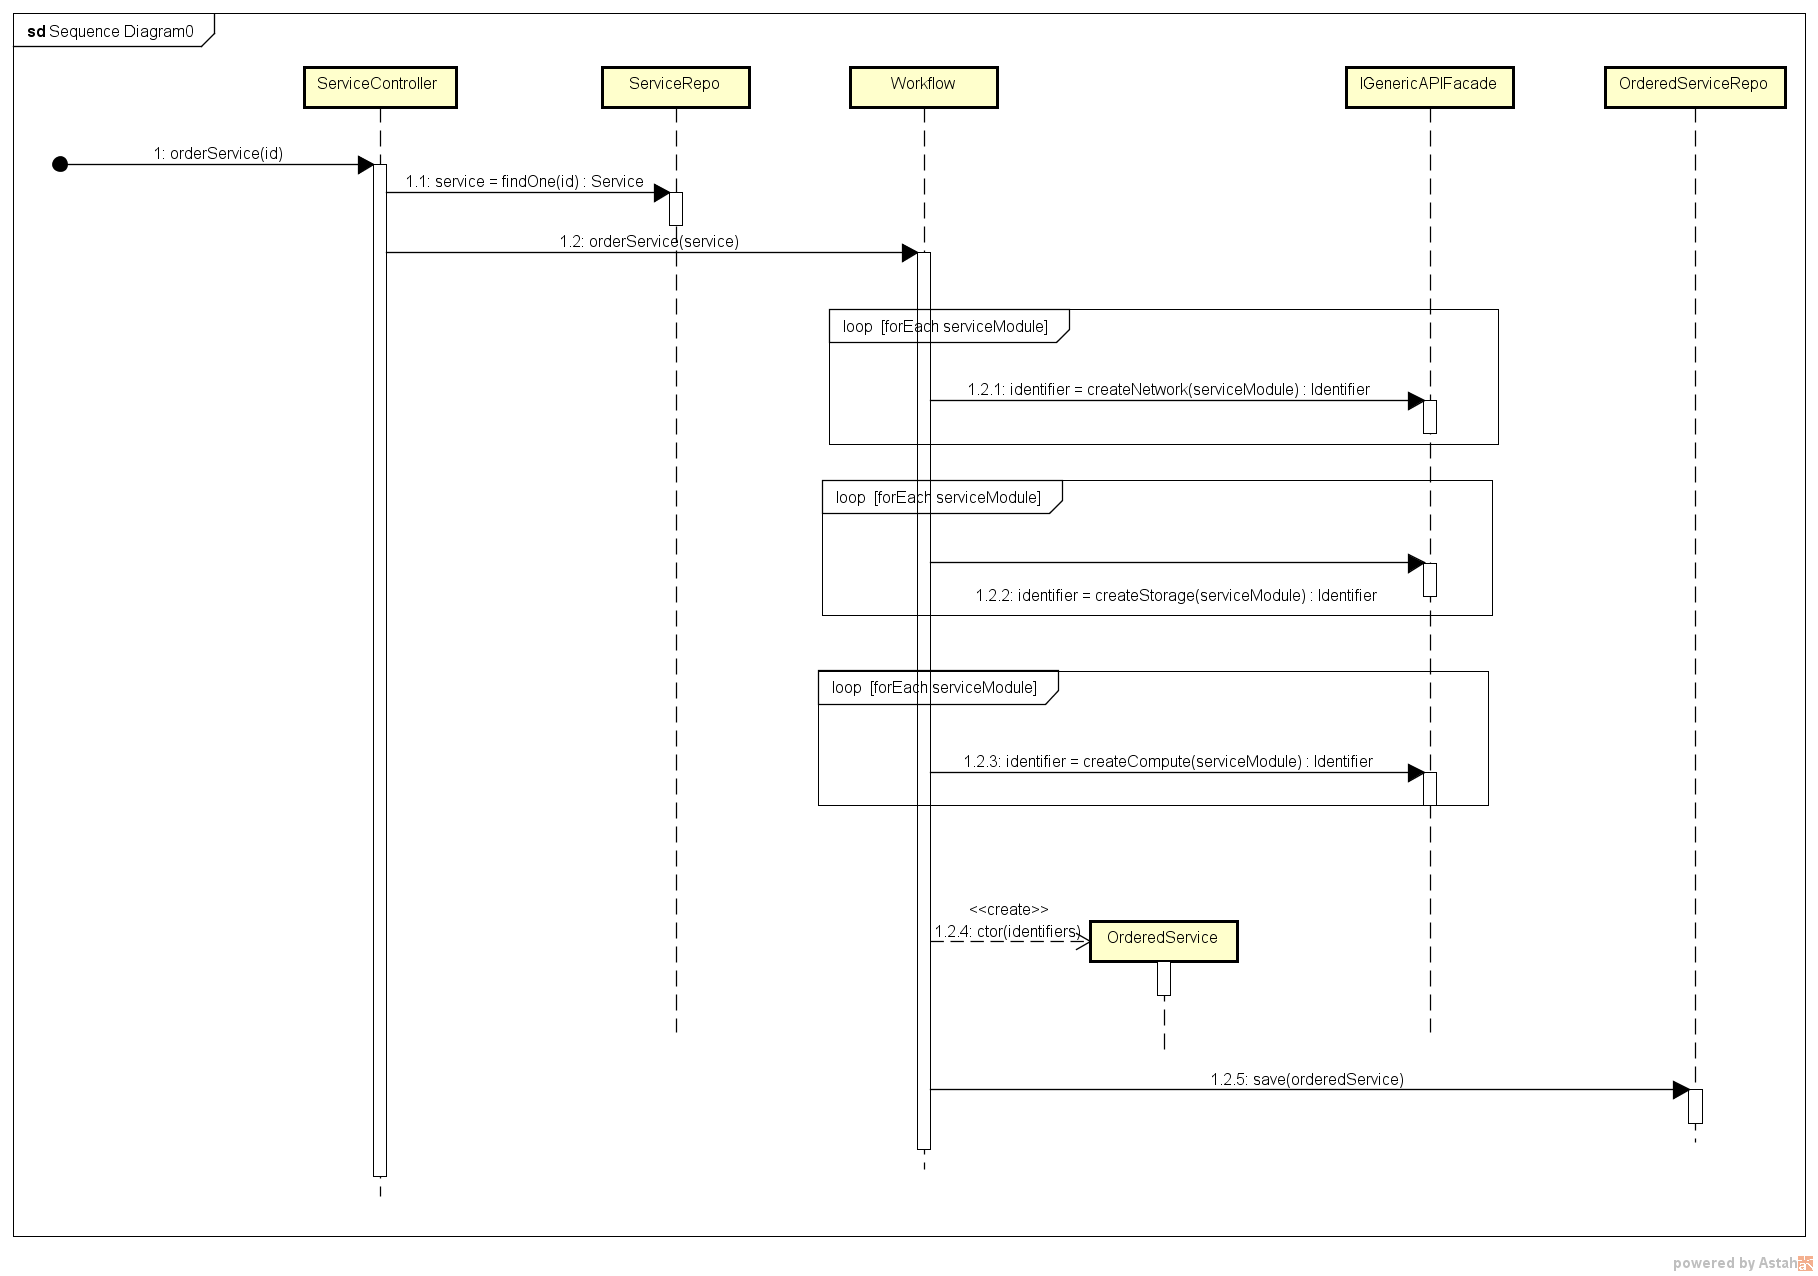
\includegraphics[width=\textwidth]{./05_Design/04_Architektur/orderService}
\end{center}
